\documentclass[12pt]{article}
\setlength{\oddsidemargin}{0in}
\setlength{\evensidemargin}{0in}
\setlength{\textwidth}{6.5in}
\setlength{\parindent}{0in}
\setlength{\parskip}{\baselineskip}

\usepackage{amsmath,amsfonts,amssymb,bm,graphics,pgfplots,framed,dsfont}
\usepackage[scale=0.75,top=1cm,bottom=3cm]{geometry}

\begin{document}

\textbf{Minh Anh Nguyen }\\
\textbf{Calculus 1 Assignment-6}\\
\textbf{Section: 04}\\
\textbf{TA's name: Arthur Huey}

\hrulefill

Section 3.1:

\begin{enumerate}
    \setcounter{enumi}{34}
    \item Find the critical numbers of the function.\\
        \[g(y) = \frac{y-1}{y^2-y+1}\]
        \[g'(y) = \frac{(y-1)'(y^2-y+1) - (y^2-y+1)'(y-1)}{(y^2-y+1)^2}\]
        \[g'(y) = \frac{y^2-y+1 - (2y-1)(y-1)}{(y^2-y+1)^2}\]
        \[g'(y) = \frac{y^2-y+1 - 2y^2+2y+y-1}{(y^2-y+1)^2}\]
        \[g'(y) = \frac{-y^2+2y}{(y^2-y+1)^2}\]
        \[-y^2+2y=0\]
        \[-y(y-2)=0\]
        \[y = 0 \text{ or } y = 2\]
        The critical numbers of the function are 0 and 2.
    \setcounter{enumi}{40}
    \item Find the critical numbers of the function.
        \[F(x) = x^{4/5}(x-2)^2\]
        \[F(x) = x^{4/5}(x^2-4x+4)\]
        \[F(x) = x^{14/5}-4x^{9/5}+4x^{4/5}\]
        \[F'(x) = \frac{14}{5}x^{9/5}-\frac{36}{5}x^{4/5}+\frac{16}{5}x^{-1/5}\]
        \[\frac{14}{5}x^{9/5}-\frac{36}{5}x^{4/5}+\frac{16}{5}x^{-1/5}=0\]
        \[x = \frac{4}{7} \text{ or } x = 2\]
        The critical numbers of the function are ${\displaystyle \frac{4}{7}}$ and 2.
    \newpage
    \setcounter{enumi}{44}
    \item Find the critical numbers of the function.
        \[f(\theta) = 2\cos\theta + \sin^2\theta\]
        \[f'(\theta) = -2\sin\theta + 2\sin\theta\cos\theta\]
        \[0 = -2\sin\theta + 2\sin\theta\cos\theta\]
        \[2\sin\theta = 2\sin\theta\cos\theta\]
        \[\theta = n\pi \text{ with n is a integer.}\]
        The critical numbers of the function are $n\pi$ with n is a integer.
    \setcounter{enumi}{52}
    \item Find the absolute maximum and absolute minimum values of $f$ on the given interval.
        \[f(x)=3x^4-4x^3-12x^2+1\text{, [-2,3]}\]
        \[f'(x)=12x^3-12x^2-24x\]
        \[12x^3-12x^2-24x=0\]
        \[12x(x^2-x-2)=0\]
        \[12x(x-2)(x+1)=0\]
        \[x = 0 \text{ or } x = 2 \text{ or } x=-1\]
        \[f(-2) = 33\]
        \[f(-1) = -4\]
        \[f(0) = 1\]
        \[f(2) = -31\]
        \[f(3) = 28\]
        The absolute maximum value of $f$ is 33 and the absolute minimum value of $f$ is -31.
    \setcounter{enumi}{58}
    \item Find the absolute maximum and absolute minimum values of $f$ on the given interval.
        \[f(t) = 2\cos t + \sin 2t, [0,\frac{\pi}{2}]\]
        \[f'(t) = -2\sin t + 2\cos 2t\]
        \[0 = -2\sin t + 2\cos 2t\]
        \[2\cos 2t = 2\sin t\]
        \[\cos 2t = \cos (\frac{\pi}{2} - t)\]
        \[2t = \frac{\pi}{2} - t\]
        \[3t = \frac{\pi}{2}\]
        \[t = \frac{\pi}{6}\]
        \[f(0) = 2\]
        \[f(\frac{\pi}{6}) = \frac{3\sqrt{3}}{2}\]
        \[f(\frac{\pi}{2}) = 0\]
        The absolute maximum value of $f$ is ${\displaystyle \frac{3\sqrt{3}}{2}}$ and the absolute minimum value of $f$ is 0.
\end{enumerate}

\newpage
Section 3.2:
\begin{enumerate}
    \setcounter{enumi}{6}
    \item The graph of a function $f$ is shown. Does $f$ satisfy the hypotheses of the Mean Value Theorem on the interval $[0,5]$? If so, find a value $c$ that satisfies the conclusion of the Mean Value Theorem on that interval.
        \begin{center}
            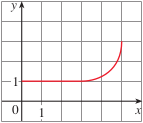
\includegraphics{img/img-0.png}    
        \end{center}    
    Based on the graph, $f$ is both continuous on the interval $[0,5]$ and differentiable on the interval $(0,5)$.
        \[f'(c) = \frac{f(5) - f(0)}{5-0}\]
        \[f'(c) = \frac{3 - 1}{5}\]
        \[f'(c) = \frac{2}{5}\]
    Based on the graph:
        \[c \approx 4\]
    \setcounter{enumi}{10}
    \item Verify that the function satisfies the three hypotheses of Rolle’s Theorem on the given interval. Then find all numbers $c$ that satisfy the conclusion of Rolle’s Theorem.
        \[f(x) = \sin (x/2) \text{, }[\frac{\pi}{2},\frac{3\pi}{2}]\]
    Because $f(x)$ is a trigonometric function, $f(x)$ is both continuous on the interval $[\frac{\pi}{2},\frac{3\pi}{2}]$ and differentiable on the interval $(\frac{\pi}{2},\frac{3\pi}{2})$.
        \[f(\frac{\pi}{2}) = \sin (\pi/4) = \frac{\sqrt{2}}{2}\]
        \[f(\frac{3\pi}{2}) = \sin (3\pi/4) = \frac{\sqrt{2}}{2}\]
    Hence, $f(\frac{\pi}{2}) = f(\frac{3\pi}{2}) = \frac{\sqrt{2}}{2}$. Therefore, there exists $c$ in $(\frac{\pi}{2},\frac{3\pi}{2})$ such as:
        \[f'(c) = 0\]
        \[\frac{1}{2} \cos(c/2) = 0\]
        \[\cos(c/2) = 0\]
        \[c/2 = \pi/2 + k\pi \text{ with k is a integer.}\]
        \[c = \pi + 2k\pi \text{ with k is a integer.}\]
        Therefore, in the interval $(\frac{\pi}{2},\frac{3\pi}{2})$, the only $c$ satisfies the conclusion of Rolle’s Theorem is $\pi$.
        \setcounter{enumi}{12}
        \newpage
    \item Let $f(x) = 1 - x^{2/3}$. Show that $f(-1) = f(1)$ but there is no number $c$ in $(-1,1)$ such that $f'(c) = 0$. Why does this not contradict Rolle’s Theorem?\\
    Firstly, $f(x)$ is continuous on the interval $[-1,1]$.    
        \[f'(x) = -\frac{2}{3}x^{-1/3}\]
        \[f'(x) = -\frac{2}{3\sqrt[3]{x}}\]
    But $f(x)$ is not differentiable with x = 0.\\
    Therefore, this function cannot contradict with Rolle’s Theorem.
    \setcounter{enumi}{16}
    \item Verify that the function satisfies the hypotheses of the Mean Value Theorem on the given interval. Then find all numbers $c$ that satisfy the conclusion of the Mean Value Theorem.
        \[f(x) = \sqrt[3]{x}\text{, } [0,1]\] 
        \[f(x) = x^{1/3}\]
        \[f'(x) = \frac{1}{3}x^{-2/3}\]
    Firstly, f(x) is continuous on the interval [0,1].\\
    Secondly, f(x) is differentiable on the integer (0,1).
    Then there is a number $c$ in (0,1) such that:
        \[f'(c) = \frac{f(1) - f(0)}{1-0}\]
        \[\frac{1}{3}c^{-2/3} = \frac{1 - 0}{1 - 0}\]
        \[\frac{1}{3}c^{-2/3} = 1\]
        \[c = \frac{\sqrt{3}}{9}\]
    \setcounter{enumi}{20}
    \item Let $f(x) = (x-3)^{-2}$. Show that there is no value of $c$ in (1,4) such that $f(4) - f(1) = f'(c)(4-1)$. Why does this not contradict the Mean Value Theorem?
        \[f(x) = (x-3)^{-2}\]
        \[f(x) = \frac{1}{(x-3)^{2}}\]
        The function $f(x)$ is not defined at x =3. Therefore, it's not continuous on x = 3 in the inteval (1,4). Hence, it does not contradict the Mean Value Theorem.
    \setcounter{enumi}{22}
    \item Show that the equation has exactly one real solution.
        \[2x + \cos x = 0\]
    Let say:
        \[f(x) = 2x + \cos x\]
        \[f'(x) = 2 - \sin x\]
    Because:
        \[-1 < \sin x < 1\]
        \[1 > -\sin x > -1\]
        \[3 > 2-\sin x > 1\]
        \[3 > f'(x) > 1\]
    Because f'(x) is always positive, the function is always increasing.\\
    For x = 0:
        \[f(0) = 1 > 0\] 
    For x = -1:
        \[f(-1) \approx -1.46 < 0 \] 
    Therefore, f(x) has a root between (-1,0) and because f(x) is always increasing. f(x) only has one real solution.
    \setcounter{enumi}{24}
    \item Show that the equation $x^3 - 15x + c = 0$ has at most one solution in the interval [-2,2].
\end{enumerate}

Section 3.3:


\begin{enumerate}
    \setcounter{enumi}{5}
    \item The graph of the derivative $f'$ of a function $f$ is shown.
    \begin{center}
        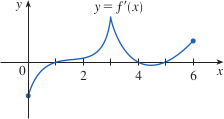
\includegraphics{img/img-1.png}
    \end{center}
    \begin{enumerate}
        \item On what intervals is $f$ increasing? Decreasing?\\
        $f$ is increasing on the intervals (1,4),(5,6).\\
        $f$ is decreasing on the intervals (0,1),(4,5).
        \item At what values of $x$ does $f$ have a local maximum? Local minimum?\\
        $f$ has local maximum at x = 4.\\
        $f$ has local minimum at x = 1, and x = 5.
    \end{enumerate}
    \item In each part use the given graph to state the $x$-coordinates of the inflection points of $f$. Give reasons for your answers.
    \begin{center}
        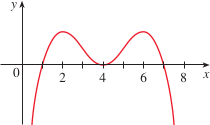
\includegraphics{img/img-2.png}
    \end{center}
    \begin{enumerate}
        \item The curve is the graph of $f$.\\
        The inflection points are 3, 5.
        \item The curve is the graph of $f'$.\\
        The inflection points are 2, 4, 6.
        \item The curve is the graph of $f''$.\\
        The inflection points are 1, 7.
    \end{enumerate}
    \setcounter{enumi}{8}
    \item Find the intervals on which $f$ is increasing or decreasing, and find the local maximum and minimum values of $f$.
        \[f(x) = 2x^3 - 15x^2 + 24x - 5\]
        \[f'(x) = 6x^2 - 30x + 24\]
        \[6x^2 - 30x + 24 = 0\]
        \[x = 1 \text{ or } x = 4\]\\
        Function f(x) is increasing in the intervals $(-\infty, 1)$ and $(4, \infty)$\\
        Function f(x) is decreasing in the intervals $(1,4)$.\\
        The local maximum of the function is f(x) with x = 1.\\
        The local minimum of the function is f(x) with x = 4.
    \setcounter{enumi}{12}
    \item Find the intervals on which $f$ is increasing or decreasing, and find the local maximum and minimum values of $f$.
        \[f(x) = \frac{x^2-24}{x-5}\]
        \[f'(x) = \frac{(x^2-24)'(x-5) - (x-5)'(x^2-24)}{(x-5)^2}\]
        \[f'(x) = \frac{(2x)(x-5) - x^2 + 24}{(x-5)^2}\]
        \[f'(x) = \frac{2x^2 - 10x - x^2 + 24}{(x-5)^2}\]
        \[f'(x) = \frac{x^2 - 10x + 24}{(x-5)^2}\]
        \[x^2 - 10x + 24 = 0\]
        \[x = 4 \text{ or } x = 6\]
        Function is increasing on the intervals $(-\infty, 4)$ and $(6, \infty)$.\\
        Function is decreasing on the interval $(4,6)$.\\
        The local maximum of the function is f(x) with x = 4.\\
        The local minimum of the function is f(x) with x = 6.
        \setcounter{enumi}{16}
        \newpage
    \item Find the intervals on which $f$ is concave upward or concave downward, and find the infection points of $f$.
        \[f(x) = \sin^2(x) - \cos 2x \text{, } 0 \leq x \leq \pi\]
        \[f'(x) = 2\sin(x)\cos(x) + 2\sin 2x\]
        \[f''(x) = 2[(\sin(x))'\cos(x) + \sin(x)(\cos(x))'] + 4\cos 2x\]
        \[f''(x) = 2[\cos^2(x) - \sin^2(x)] + 4\cos 2x\]
        \[f''(x) = 2\cos^2(x) - 2\sin^2(x) + 4(2\cos^2 x - 1)\]
        \[f''(x) = 2\cos^2(x) - 2\sin^2(x) + 8\cos^2 x - 4\]
        \[f''(x) = 2\cos^2(x) - 2\sin^2(x) + 8\cos^2 x - 4\cos^2x - 4\sin^2x\]
        \[f''(x) = 6\cos^2(x) - 6\sin^2(x) \]
        \[6\cos^2(x) - 6\sin^2(x) = 0\]
        \[6\cos^2(x) = 6\sin^2(x)\]
        \[\tan^2 x = 1\]
        \[\tan x = \pm 1\]
        Since x is in the intervals [0, $\pi$].
        \[x = \frac{\pi}{4} \text{ or } x = \frac{3\pi}{4}\]
        The inflection points of f(x) are $(\frac{\pi}{4}, \frac{1}{2})$ and $(\frac{3\pi}{4}, \frac{1}{2})$.\\
        The function f(x) is concave up in the intervals $(0,\frac{\pi}{4})$ and $(\frac{3\pi}{4},\pi)$.\\
        The function f(x) is concave down in the interval $(\frac{\pi}{4}, \frac{3\pi}{4})$
        \setcounter{enumi}{21}
    \item \[f(x) = \cos^2x - 2\sin x \text{, } 0 \leq x \leq 2\pi\]
        \begin{enumerate}
            \item Find the intervals on which $f$ is increasing or decreasing.
                \[f'(x) = -2\cos x \sin x - 2\cos x\]
                \[-2\cos x \sin x - 2\cos x = 0\]
                \[-2\cos x(\sin x + 1) = 0\]
                \[\cos x = 0 \text{ or } \sin x + 1 = 0\]
                \[ x = \pi/2 + \pi n \text{ with n is a integer or } \sin x = -1\]
                \[ x = \pi/2 + \pi n \text{ or } x = 3\pi/2 + 2\pi n \text{ with n is a integer.}\]
                Since x is in the inteval $[0,2\pi]$.
                \[x \in \{\pi/2,3\pi/2\}\]
                The function $f(x)$ is increasing on the intevals $(\pi/2,3\pi/2)$.\\
                The function $f(x)$ is decreasing on the intevals $(0,\pi/2)$ and $(3\pi/2,2\pi)$.
            \item Find the local maximum and minimum values of $f$.\\
                The local maximum value of $f$ is: $f(3\pi/2) = 2$.\\
                The local minimum value of $f$ is: $f(\pi/2) = -2$
            \item Find the intervals of concavity and the inflection points.
                \[f''(x) = -2(-\sin^2 x + \cos^2 x) - 2\cos x\]
                \[f''(x) = 2\sin^2 x -2\cos^2 x - 2\cos x\]
                \[2\sin^2 x -2\cos^2 x - 2\cos x = 0\]
                \[x \in \{\pi/3,\pi,5\pi/3\}\]
                The inflection points are $(\pi/3, \frac{1-4\sqrt{3}}{4}), (\pi,1), (5\pi/3, \frac{1+4\sqrt{3}}{4})$.\\
                The function is concave up in the interval $(\pi/3,\pi)$.\\
                The function is concave down in the interval $(0,\pi/3)$ and $(5\pi/3,2\pi)$
        \end{enumerate}
        \item Find the local maximum and minimum values of $f$ using both the First and Second Derivative Tests. Which method do you prefer?
            \[f(x) = 1 + 3x^2 - 2x^3\]
            \[f'(x) = 6x - 6x^2\]
            \[f''(x) = 6 - 12x\]
        The First Derivative Test:

\end{enumerate}

\end{document}